\documentclass[11pt]{charter}

% El títulos de la memoria, se usa en la carátula y se puede usar el cualquier lugar del documento con el comando \ttitle
\titulo{Implementación de Interfaz SDI en FPGA Cyclone V} 

% Nombre del posgrado, se usa en la carátula y se puede usar el cualquier lugar del documento con el comando \degreename
\posgrado{Carrera de Especialización en Sistemas Embebidos} 
%\posgrado{Carrera de Especialización en Internet de las Cosas} 
%\posgrado{Carrera de Especialización en Intelegencia Artificial}
%\posgrado{Maestría en Si%stemas Embebidos} 
%\posgrado{Maestría en Internet de las cosas}

% Tu nombre, se puede usar el cualquier lugar del documento con el comando \authorname
\autor{Joaquin Gaspar Ulloa} 

% El nombre del director y co-director, se puede usar el cualquier lugar del documento con el comando \supname y \cosupname y \pertesupname y \pertecosupname
\director{Diego Marcelo Martin}
\pertenenciaDirector{MPS} 
% FIXME:NO IMPLEMENTADO EL CODIRECTOR ni su pertenencia
\codirector{} % si queda vacio no se deberíá incluir 
\pertenenciaCoDirector{}

% Nombre del cliente, quien va a aprobar los resultados del proyecto, se puede usar con el comando \clientename y \empclientename
\cliente{Marcelo Indarramendi}
\empresaCliente{VideoSwitch}

% Nombre y pertenencia de los jurados, se pueden usar el cualquier lugar del documento con el comando \jurunoname, \jurdosname y \jurtresname y \perteunoname, \pertedosname y \pertetresname.
\juradoUno{Nombre y Apellido (1)}
\pertenenciaJurUno{pertenencia (1)} 
\juradoDos{Nombre y Apellido (2)}
\pertenenciaJurDos{pertenencia (2)}
\juradoTres{Nombre y Apellido (3)}
\pertenenciaJurTres{pertenencia (3)}
 
\fechaINICIO{23 de Octubre de 2020}		%Fecha de inicio de la cursada de GdP \fechaInicioName
\fechaFINALPlanificacion{11 de diciembre de 2020} 	%Fecha de final de cursada de GdP
\fechaFINALTrabajo{22 de agosto de 2021}		%Fecha de defensa pública del trabajo final

\begin{document}

\maketitle
\thispagestyle{empty}
\pagebreak


\thispagestyle{empty}
{\setlength{\parskip}{0pt}
\tableofcontents{}
}
\pagebreak


\section{Registros de cambios}
\label{sec:registro}


\begin{table}[ht]
\label{tab:registro}
\centering
\begin{tabularx}{\linewidth}{@{}|c|X|c|@{}}
\hline
\rowcolor[HTML]{C0C0C0} 
Revisión & \multicolumn{1}{c|}{\cellcolor[HTML]{C0C0C0}Detalles de los cambios realizados} & Fecha      \\ \hline
1.0      & Creación del documento                                          & 23/10/2020 \\ \hline
1.1      & Avances hasta entregables principales del proyecto & 06/11/2020 \\ \hline
1.2      & Se agregan historias de usuarios y se hacen correcciones & 15/11/2020 \\ \hline
%1.2      & Otro ejemplo \newline
%		   Con texto partido \newline
%		   En varias líneas \newline
%		   A propósito                                                     & dd/mm/aaaa \\ \hline
\end{tabularx}
\end{table}

\pagebreak

\section{Acta de constitución del proyecto}
\label{sec:acta}

\begin{flushright}
Buenos Aires, \fechaInicioName
\end{flushright}

\vspace{2cm}

Por medio de la presente se acuerda con el Ing. \authorname\hspace{1px} que su Trabajo Final de la \degreename\hspace{1px} se titulará ``\ttitle'', consistirá esencialmente en un módulo de procesamiento serie digital, como remplazo del IP-SDI-II Core de Intel, capaz de transmitir, recibir y procesar tanto los datos entregados por el cable drivers, como por el core de la FPGA y tendrá un presupuesto preliminar estimado de 704 hs de trabajo y \textcolor{red}{\$XXX}, con fecha de inicio \fechaInicioName\hspace{1px} y fecha de presentación pública \fechaFinalName.

Se adjunta a esta acta la planificación inicial.

\vfill

% Esta parte se construye sola con la información que hayan cargado en el preámbulo del documento y no debe modificarla
\begin{table}[ht]
\centering
\begin{tabular}{ccc}
\begin{tabular}[c]{@{}c@{}}Ariel Lutenberg \\ Director posgrado FIUBA\end{tabular} & \hspace{2cm} & \begin{tabular}[c]{@{}c@{}}\clientename \\ \empclientename \end{tabular} \vspace{2.5cm} \\ 
\multicolumn{3}{c}{\begin{tabular}[c]{@{}c@{}} \supname \\ Director del Trabajo Final\end{tabular}} \vspace{2.5cm} \\
%\begin{tabular}[c]{@{}c@{}}\jurunoname \\ Jurado del Trabajo Final\end{tabular}     &  & \begin{tabular}[c]{@{}c@{}}\jurdosname\\ Jurado del Trabajo Final\end{tabular}  \vspace{2.5cm}  \\
%\multicolumn{3}{c}{\begin{tabular}[c]{@{}c@{}} \jurtresname\\ Jurado del Trabajo Final\end{tabular}} \vspace{.5cm}                                                                     
\end{tabular}
\end{table}


\section{Descripción técnica-conceptual del proyecto a realizar}
\label{sec:descripcion}


En este proyecto se busca desarrollar un módulo SDI (del inglés Serial Digital Interface) para reemplazar el módulo que se utiliza actualmente, que es un IP (del inglés Intellectual Property) Core de Intel, lo que implica que es pago y está sujeto a una versión del IDE de desarrollo. Se busca implementar una interfaz bidireccional conformada por dos partes principales, la física y la de protocolo.

Uno de los principales objetivos de este desarrollo es que mediante un módulo de FPGA auto contenido la empresa pueda dar un paso hacia la independencia tecnológica en los productos que desarrolla. Este aspecto es de vital importancia, ya que los productos de la empresa se encuentran en constante desarrollo y muchas veces la dependencia de alguna plataforma de desarrollo o propiedad intelectual generan demoras en los desarrollos y hasta limitaciones a la hora de implementar nuevas tecnologías. Se considera que esta idea va en la misma linea de pensamiento, que la misión de la empresa:

"Diseñar y desarrollar equipamiento, desde la excelencia, tanto en Hardware como en Software, de tal forma que permitan cubrir las necesidades de nuestros clientes y agregar valor a sus servicios de Televisión estableciendo una comunicación que nos permita una mejora continua a través de producciones de alta tecnología apuntando a establecer una red de comercialización global en un futuro cercano."

Los principales aspectos técnicos de este trabajo se pueden agrupar en dos. Por un lado, los conocimientos sobre el estándar de comunicación y sus aplicaciones, donde tendrá un rol central la experiencia con la que cuenta la empresa. Por otro lado, la experiencia en desarrollos en FPGA, particularmente en aplicaciones para TV digital, donde será clave la opinión del director.

En lo referido al estándar es importante contextualizar su área de aplicación. En el ambiente de la televisión es muy común tener que transmitir señales digitales no comprimidas y por medios compatibles con los medios analógicos. Con tal fin, muchos equipos de televisión digital cuentan con interfaces SDI, para transmitir señales de alta calidad.
El estándar SDI, creado por la SMPTE en 1989, es una interfaz digital serie asincrónica, cuya principal aplicación es la transmisión de señales de video digital profesional no comprimido y no encriptado, por cables coaxiales de 75 ohm. Este estándar tiene como principal característica que admite muy alto bitrate y no agrega grandes retardos.

\vspace{25px}

\begin{figure}[htpb]
\centering 
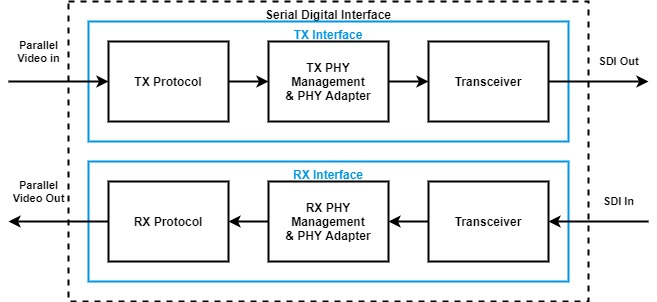
\includegraphics[width=.7\textwidth]{./Figuras/SDI.jpg}
\caption{Diagrama en bloques de la interfaz SDI}
\label{fig:diagBloques}
\end{figure}

\vspace{25px}

En cuanto a la implementación en FPGA, la interfaz SDI consta de dos capas independientes, que se pueden visualizar en la Figura \ref{fig:diagBloques}, la de recepción/transmisión y la de protocolo, por tal motivo el módulo deberá implementar ambas instancias de manera separada. Para la primera se suelen usar hard-transceivers, contenidos en la FPGA o soft-transceivers instanciados con lógica, para las aplicaciones con menor demanda de bitrate. Este módulo se encarga de muestrear la entrada asincrónica, sincronizarse a la misma y deserializar los datos. Para la segunda etapa, se debe implementar un submódulo que trabaje en el dominio de los datos paralelizados y tenga la información propia del protocolo para interpretar, acondicionar y validar la señal. Esta parte del desarrollo se encarga principalmente de la sincronización de paquetes y de la detección de errores.
Aunque la interfaz funciona en un solo sentido, debe ser configurable para funcionar como transmisor y receptor de manera separada, como se ilustra en la Figura \ref{fig:diagBloques}. Por lo tanto, el módulo a desarrollar debe ser capaz de tomar la señal serie que llega a la FPGA desde el driver del cable, deserializarla y procesarla en un sentido y paquetizar la señal acorde al protocolo y serializarla en el otro sentido.

Debido a la creciente demanda de procesamiento y consiguientemente el mayor uso de recursos en la FPGA, debe diseñarse el módulo de forma tal que solo se instancie lo mínimo indispensable, para el funcionamiento en el formato que se configure, ya sea por el sentido de los datos o el bitrate de los mismo.

El desarrollo debe estar pensado para su implementación sobre el hardware de los equipos de la empresa, que ya cuenta con un driver apropiado para tal fin y un microcontrolador capaz de controlar el módulo. Por tal motivo, la implementación debe hacerse con una FPGA Cyclone V de Intel, que son las que usan los equipos más modernos de la empresa, pero en lo posible debe ser independiente del modelo de dispositivo a usar, para asegurar portabilidad.

\section{Identificación y análisis de los interesados}
\label{sec:interesados}

\begin{table}[ht]
%\caption{Identificación de los interesados}
%\label{tab:interesados}
\begin{tabularx}{\linewidth}{@{}|l|X|X|l|@{}}
\hline
\rowcolor[HTML]{C0C0C0} 
Rol           & Nombre y Apellido & Organización 	& Puesto 	\\ \hline
Auspiciante   & Roberto Maury     &\empclientename 	& CEO    	\\ \hline
Cliente       & \clientename      &\empclientename	& Development Engineering Manager \\ \hline
%Impulsor      &                   &              	&        	\\ \hline
Responsable   & \authorname       & FIUBA        	& Alumno 	\\ \hline
%Colaboradores &                   &              	&        	\\ \hline
Orientador    & \supname	      & \pertesupname 	& Director	Trabajo final \\ \hline
%Equipo        & miembro1 \newline 
%				miembro2          &              	&        	\\ \hline
%Opositores    &                   &              	&        	\\ \hline
%Usuario final &                   &              	&        	\\ \hline
\end{tabularx}
\end{table}

\begin{itemize}
\item Auspiciante: Roberto, promueve los desarrollos y las capacitaciones, es exigente con el cumplimiento de los horarios y las normas.
\item Cliente: Marcelo, tiene gran conocimiento en el desarrollo de proyectos, conoce los equipos de la empresa y las normas de TV digital.
\item Orientador: Diego, tiene amplio conocimiento sobre desarrollos en FPGA y buen manejo de normas de TV digital.
\end{itemize}

\section{1. Propósito del proyecto}
\label{sec:proposito}

El propósito de este proyecto es realizar una interfaz SDI para FPGA con la capacidad de transmitir y recibir señales de video digital de alto bitrate, para en un futuro utilizarlo tanto en los equipos que actualmente comercializa la empresa, así como también en futuros desarrollos.

\section{2. Alcance del proyecto}
\label{sec:alcance}

En este proyecto se diseñará e implementará la descripción de los circuitos digitales en lenguaje VHDL para implementar en una FPGA Cyclone V, cuya funcionalidades serán tanto recibir y decodificar como serializar y transmitir datos entre una interfaz SDI y el core de procesamiento de la FPGA. Del lado de la FPGA la información será entragada en palabras, cuyo largo y bitrate será acordado con el cliente.

Se incluirán los archivos complementarios necesarios para el correcto funcionamiento del módulo, ya sean SDC o scripts de TCL del proyectos. Además, se incluirá la documentación del diseño y para la operación del módulo por una persona capacitada.

El control de la configuración del módulo será por medio en una interfaz SPI-Avalon ya implementada en VHDL.

En el presente proyecto no se incluirán ningún tipo de diseño ni implementación de hardware o firmware complementaria al diseño. El diseño no cumplirá con estándares SDI con tasas de bitrate superiores a los 3 Gbit/s.

\section{3. Supuestos del proyecto}
\label{sec:supuestos}

Para el desarrollo del presente proyecto se supone que:

\begin{itemize}
\item Se cuenta con el hardware necesario para su implementación, con driver SDI y una FPGA Cyclone V con hard-transceivers.
\item Se cuenta con los instrumentos de medición necesarios.
\item Se cuenta con las licencias de software necesarias para el desarrollo.
\item Se cuenta con el módulo que se desea remplazar.
\item Se cuenta con el tiempo necesario dentro de la empresa para hacer el desarrollo y las pruebas.
\item Se cuenta con las normas en cuestión.
\end{itemize}

\section{4. Requerimientos}
\label{sec:requerimientos}

\begin{enumerate}
\item Validación
	\begin{enumerate}
	\item Medición y observación de audio y video luego de pasar por el sistema completo.
	\item Medición de los los paquetes con un analizador según la norma.
	\item Cumplir con el bitrate de los estándares dentro del rango de SD-SDI y 3G-SDI.
	\end{enumerate}
\item Funcionalidad
	\begin{enumerate}
	\item Obtener las tasas de bitrate contempladas dentro del rango de los estandares SD-SDI y 3G-SDI.
	\item Obtener un diseño sin problemas de timing en las señales entre dominios de clock dentro del módulo.
	\item Obtener un módulo sin problemas de timing por setup o hold en las señales de entrada y salida.
	\item La implementación del sistema no debe ocupar más del 3000 Logic Array Blocks en la FPGA.
	\end{enumerate}
\item Metodología de trabajo
	\begin{enumerate}
	\item Control de versiones mediante SVN.
	\item Desarrollo en Quartus con licencias para análisis de timing y simulaciones.
	\item Planificación y documentación mediante Redmine.
	\item Diseño modular.
	\end{enumerate}
\item Documentación
	\begin{enumerate}
	\item Confección de la memoria técnica.
	\item Confección de documentación del diseño del módulo.
	\item Confección de documentación de uso del módulo.
	\end{enumerate}
\end{enumerate}

\section{Historias de usuarios (\textit{Product backlog})}
\label{sec:backlog}


\begin{itemize}
\item Como desarrollador de hardware, necesito que la interfaz SDI se comunique con el driver mediante un puerto LVDS, para no tener que modificar la placa. Story point: 1
\item Como desarrollador de firmware, necesito poder configurar el módulo escribiendo registro de 32 bits, para que se maneje de la misma manera que los demás módulos de FPGA. Story point: 1
\item Como desarrollador de firmware, necesito que el microcontrolador se comunique con el módulo mediante una interfaz SPI común a toda a FPGA, para no tener que modificar el driver. Story point: 2
\item Como encargado del producto Encoder, necesito que la interfaz soporte tasas de datos compatibles al menos con videos de calidad HD, para recibir video no comprimido. Story point: 13
\item Como supervisor de desarrollo, necesito que la interfaz soporte videos de calidad 3G o por lo menos permita la posibilidad de hacer el desarrollo a futuro, para futuros desarrollos. Story point: 40
\item Como supervisor de desarrollo, necesito que el módulo use los clock y señales actualmente disponibles, para que sea retrocompatible. Story point: 3
\item Como supervisor de desarrollo, necesito que el módulo funcione en Cyclone V y en las configuraciones que sea posible lo haga sin hard-transceivers, para poder abaratar costos cuando sea posible. Story point: 13
\item Como encargado del producto Encoder, necesito que el módulo sea compatible con paquetes de transport stream de 188 Bytes y 204 Bytes, para poder ser usado en distintas etapas de la cadena transmisión de TV digital. Story point: 8
\end{itemize}

El story point de cada historia de usuario fue definido según un formato similar a la serie de Fibonacci, tomando los valores: 0, 0.5, 1, 2, 3, 5, 8, 13, 20, 40, 100. Contemplando la complejidad de la tarea con un peso de 0.3, el volumen de la misma con un peso de 0.25, la incertidumbre con un peso de 0.35 y potenciales riesgos con un peso de 0.1, sobre un total unitario. El conocimiento del equipo está implícito en las otras cuatro categorías dado que de momento soy el único integrante.

\section{5. Entregables principales del proyecto}
\label{sec:entregables}

\begin{itemize}
\item Diseño en VHDL y archivos complementarios.
\item Manual de implementación.
\item Diagrama esquemático y memoria de decisiones de diseño.
\item Informes de avances mediante tareas de Redmine.
\item Informe final.
\end{itemize}

\section{6. Desglose del trabajo en tareas}
\label{sec:wbs}

\begin{enumerate}
\item Investigación preliminar (56 hs)
	\begin{enumerate}
	\item Búsqueda de documentación, material y desarrollos. (8 hs)
	\item Estudio de normas. (8 hs)
	\item Estudio de hojas de datos de componentes con esta funcionalidad. (4 hs)
	\item Estudio de desarrollos similares. (12 hs)
	\item Estudio de documentación de productos similares. (20 hs)
	\item Discutir resultados obtenidos con el director y el cliente. (4 hs)
	\end{enumerate}
\item Planificación (12 hs)
	\begin{enumerate}
	\item Planificación de tareas. (8 hs)
	\item Documentación de la planificación. (4 hs)
	\end{enumerate}
\item Diseño (116 hs)
	\begin{enumerate}
	\item Definición parámetros de diseño. (20 hs)
	\item Definición de interfaces del sistema. (12 hs)
	\item Diseño del diagrama en bloques. (16 hs)
	\item Investigar que módulos ya se encuentran desarrollados. (4 hs)
	\item Diseño detallado de los bloques. (40 hs)
	\item Definición de pruebas. (16 hs)
	\item Discutir resultados obtenidos con el director y el cliente. (8 hs)
	\end{enumerate}
\item Desarrollo (256 hs)
	\begin{enumerate}
	\item Descripción de cada módulo de la parte física de transmisión. (20 hs)
	\item Descripción de cada módulo de la parte física de recepción. (40 hs)
	\item Descripción de cada módulo de la parte del protocolo de transmisión. (40 hs)
	\item Descripción de cada módulo de la parte del protocolo de recepción. (40 hs)
	\item Integración de módulos. (40 hs)
	\item Implementación del control. (16 hs)
	\item Reuniones con el director y el cliente. (20 hs)
	\item Simulaciones. (40 hs)
	\end{enumerate}
\item Pruebas (124 hs)
	\begin{enumerate}
	\item Por módulo. (24 hs)
	\item Por bloques funcionales. (40 hs)
	\item Del sistema completo. (40 hs)
	\item Integración en equipo. (20 hs)
	\end{enumerate}
\item Documentación (140 hs)
	\begin{enumerate}
	\item Avances. (24 hs)
	\item Mediciones. (16 hs)
	\item Diseño e implementación. (40 hs)
	\item Informe Final. (40 hs)
	\item Presentación. (20 hs)
	\end{enumerate}
\end{enumerate}

Cantidad total de horas: (704 hs)

\section{7. Diagrama de Activity On Node}
\label{sec:AoN}

\begin{consigna}{red}
Armar el AoN a partir del WBS definido en la etapa anterior. 

%La figura \ref{fig:AoN} fue elaborada con el paquete latex tikz y pueden consultar la siguiente referencia \textit{online}:

%\url{https://www.overleaf.com/learn/latex/LaTeX_Graphics_using_TikZ:_A_Tutorial_for_Beginners_(Part_3)\%E2\%80\%94Creating_Flowcharts}

\end{consigna}

\begin{figure}[htpb]
\centering 
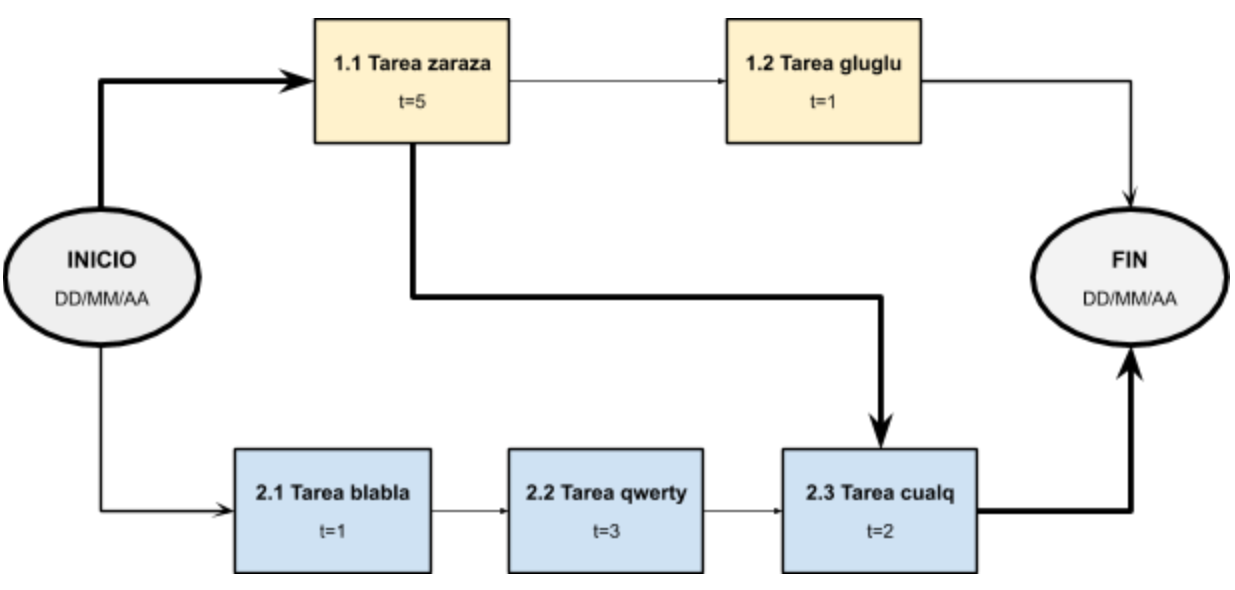
\includegraphics[width=.8\textwidth]{./Figuras/AoN.png}
\caption{Diagrama en \textit{Activity on Node}}
\label{fig:AoN}
\end{figure}

Indicar claramente en qué unidades están expresados los tiempos.
De ser necesario indicar los caminos semicríticos y analizar sus tiempos mediante un cuadro.
Es recomendable usar colores y un cuadro indicativo describiendo qué representa cada color, como se muestra en el siguiente ejemplo:



\section{8. Diagrama de Gantt}
\label{sec:gantt}

\begin{consigna}{red}
Utilizar el software Gantter for Google Drive o alguno similar para dibujar el diagrama de Gantt.

Existen muchos programas y recursos \textit{online} para hacer diagramas de gantt, entre las cuales destacamos:

\begin{itemize}
\item Planner
\item GanttProject
\item Trello + \textit{plugins}. En el siguiente link hay un tutorial oficial: \\ \url{https://blog.trello.com/es/diagrama-de-gantt-de-un-proyecto}
\item Creately, herramienta online colaborativa. \\\url{https://creately.com/diagram/example/ieb3p3ml/LaTeX}
\item Se puede hacer en latex con el paquete \textit{pgfgantt}\\ \url{http://ctan.dcc.uchile.cl/graphics/pgf/contrib/pgfgantt/pgfgantt.pdf}
\end{itemize}

Pegar acá una captura de pantalla del diagrama de Gantt, cuidando que la letra sea suficientemente grande como para ser legible. 
Si el diagrama queda demasiado ancho, se puede pegar primero la ``tabla'' del Gantt y luego pegar la parte del diagrama de barras del diagrama de Gantt.

Configurar el software para que en la parte de la tabla muestre los códigos del EDT (WBS).\\
Configurar el software para que al lado de cada barra muestre el nombre de cada tarea.\\
Revisar que la fecha de finalización coincida con lo indicado en el Acta Constitutiva.

En la figura \ref{fig:gantt}, se muestra un ejemplo de diagrama de gantt realizado con el paquete de \textit{pgfgantt}. En la plantilla pueden ver el código que lo genera y usarlo de base para construir el propio.

\begin{figure}[htbp]
\begin{center}
\begin{ganttchart}{1}{12}
  \gantttitle{2020}{12} \\
  \gantttitlelist{1,...,12}{1} \\
  \ganttgroup{Group 1}{1}{7} \\
  \ganttbar{Task 1}{1}{2} \\
  \ganttlinkedbar{Task 2}{3}{7} \ganttnewline
  \ganttmilestone{Milestone o hito}{7} \ganttnewline
  \ganttbar{Final Task}{8}{12}
  \ganttlink{elem2}{elem3}
  \ganttlink{elem3}{elem4}
\end{ganttchart}
\end{center}
\caption{Diagrama de gantt de ejemplo}
\label{fig:gantt}
\end{figure}

\end{consigna}

\section{9. Matriz de uso de recursos de materiales}
\label{sec:recursos}


\begin{table}
\label{tab:recursos}
\centering
\begin{tabularx}{\linewidth}{@{}|c|X|X|X|X|c|@{}}
\hline
\cellcolor[HTML]{C0C0C0} & \cellcolor[HTML]{C0C0C0} & \multicolumn{4}{c|}{\cellcolor[HTML]{C0C0C0}Recursos requeridos (horas)} \\ \cline{3-6} 
\multirow{-2}{*}{\cellcolor[HTML]{C0C0C0}\begin{tabular}[c]{@{}c@{}}Código\\ WBS\end{tabular}} & \multirow{-2}{*}{\cellcolor[HTML]{C0C0C0}\begin{tabular}[c]{@{}c@{}}Nombre \\ tarea\end{tabular}} & Material 1 & Material 2 & Material 3 & Material 4 \\ \hline
 &  &  &  &  &  \\ \hline
 &  &  &  &  &  \\ \hline
 &  &  &  &  &  \\ \hline
 &  &  &  &  &  \\ \hline
 &  &  &  &  &  \\ \hline
 &  &  &  &  &  \\ \hline
 &  &  &  &  &  \\ \hline
 &  &  &  &  &  \\ \hline 
 &  &  &  &  &  \\ \hline
 &  &  &  &  &  \\ \hline
 &  &  &  &  &  \\ \hline
 &  &  &  &  &  \\ \hline
 &  &  &  &  &  \\ \hline
 &  &  &  &  &  \\ \hline
 &  &  &  &  &  \\ \hline
 &  &  &  &  &  \\ \hline
 &  &  &  &  &  \\ \hline
 &  &  &  &  &  \\ \hline
 &  &  &  &  &  \\ \hline
 &  &  &  &  &  \\ \hline
 &  &  &  &  &  \\ \hline
 &  &  &  &  &  \\ \hline
 &  &  &  &  &  \\ \hline
 &  &  &  &  &  \\ \hline 
 &  &  &  &  &  \\ \hline
 &  &  &  &  &  \\ \hline
 &  &  &  &  &  \\ \hline
 &  &  &  &  &  \\ \hline

\end{tabularx}%
\end{table}


\section{10. Presupuesto detallado del proyecto}
\label{sec:presupuesto}

\begin{consigna}{red}
Si el proyecto es complejo entonces separarlo en partes:
\begin{itemize}
\item Un total global, indicando el subtotal acumulado por cada una de las áreas.
\item El desglose detallado del subtotal de cada una de las áreas.
\end{itemize}

IMPORTANTE: No olvidarse de considerar los COSTOS INDIRECTOS.

\end{consigna}

\begin{table}[htpb]
\centering
\begin{tabularx}{\linewidth}{@{}|X|c|r|r|@{}}
\hline
\rowcolor[HTML]{C0C0C0} 
\multicolumn{4}{|c|}{\cellcolor[HTML]{C0C0C0}COSTOS DIRECTOS} \\ \hline
\rowcolor[HTML]{C0C0C0} 
Descripción &
  \multicolumn{1}{c|}{\cellcolor[HTML]{C0C0C0}Cantidad} &
  \multicolumn{1}{c|}{\cellcolor[HTML]{C0C0C0}Valor unitario} &
  \multicolumn{1}{c|}{\cellcolor[HTML]{C0C0C0}Valor total} \\ \hline
 &
  \multicolumn{1}{c|}{} &
  \multicolumn{1}{c|}{} &
  \multicolumn{1}{c|}{} \\ \hline
 &
  \multicolumn{1}{c|}{} &
  \multicolumn{1}{c|}{} &
  \multicolumn{1}{c|}{} \\ \hline
\multicolumn{1}{|l|}{} &
   &
   &
   \\ \hline
\multicolumn{1}{|l|}{} &
   &
   &
   \\ \hline
\multicolumn{3}{|c|}{SUBTOTAL} &
  \multicolumn{1}{c|}{} \\ \hline
\rowcolor[HTML]{C0C0C0} 
\multicolumn{4}{|c|}{\cellcolor[HTML]{C0C0C0}COSTOS INDIRECTOS} \\ \hline
\rowcolor[HTML]{C0C0C0} 
Descripción &
  \multicolumn{1}{c|}{\cellcolor[HTML]{C0C0C0}Cantidad} &
  \multicolumn{1}{c|}{\cellcolor[HTML]{C0C0C0}Valor unitario} &
  \multicolumn{1}{c|}{\cellcolor[HTML]{C0C0C0}Valor total} \\ \hline
\multicolumn{1}{|l|}{} &
   &
   &
   \\ \hline
\multicolumn{1}{|l|}{} &
   &
   &
   \\ \hline
\multicolumn{1}{|l|}{} &
   &
   &
   \\ \hline
\multicolumn{3}{|c|}{SUBTOTAL} &
  \multicolumn{1}{c|}{} \\ \hline
\rowcolor[HTML]{C0C0C0}
\multicolumn{3}{|c|}{TOTAL} &
   \\ \hline
\end{tabularx}%
\end{table}


\section{11. Matriz de asignación de responsabilidades}
\label{sec:responsabilidades}
\begin{consigna}{red}
Establecer la matriz de asignación de responsabilidades y el manejo de la autoridad completando la siguiente tabla:

\begin{table}[htpb]
\centering
\resizebox{\textwidth}{!}{%
\begin{tabular}{|c|c|c|c|c|c|}
\hline
\rowcolor[HTML]{C0C0C0} 
\cellcolor[HTML]{C0C0C0} &
  \cellcolor[HTML]{C0C0C0} &
  \multicolumn{4}{c|}{\cellcolor[HTML]{C0C0C0}Listar todos los nombres y roles del proyecto} \\ \cline{3-6} 
\rowcolor[HTML]{C0C0C0} 
\cellcolor[HTML]{C0C0C0} &
  \cellcolor[HTML]{C0C0C0} &
  Responsable &
  Orientador &
  Equipo &
  Cliente \\ \cline{3-6} 
\rowcolor[HTML]{C0C0C0} 
\multirow{-3}{*}{\cellcolor[HTML]{C0C0C0}\begin{tabular}[c]{@{}c@{}}Código\\ WBS\end{tabular}} &
  \multirow{-3}{*}{\cellcolor[HTML]{C0C0C0}Nombre de la tarea} &
  \authorname &
  \supname &
  Nombre de alguien &
  \clientename \\ \hline
 &  &  &  &  &  \\ \hline
 &  &  &  &  &  \\ \hline
 &  &  &  &  &  \\ \hline
\end{tabular}%
}
\end{table}

{\footnotesize
Referencias:
\begin{itemize}
	\item P = Responsabilidad Primaria
	\item S = Responsabilidad Secundaria
	\item A = Aprobación
	\item I = Informado
	\item C = Consultado
\end{itemize}
} %footnotesize

Una de las columnas debe ser para el Director, ya que se supone que participará en el proyecto.
A su vez se debe cuidar que no queden muchas tareas seguidas sin ``A'' o ``I''.

Importante: es redundante poner ``I/A'' o ``I/C'', porque para aprobarlo o responder consultas primero la persona debe ser informada.

\end{consigna}

\section{12. Gestión de riesgos}
\label{sec:riesgos}

\begin{consigna}{red}
a) Identificación de los riesgos (al menos cinco) y estimación de sus consecuencias:
 
Riesgo 1: detallar el riesgo (riesgo es algo que si ocurre altera los planes previstos)
\begin{itemize}
\item Severidad (S): mientras más severo, más alto es el número (usar números del 1 al 10).\\
Justificar el motivo por el cual se asigna determinado número de severidad (S).
\item Probabilidad de ocurrencia (O): mientras más probable, más alto es el número (usar del 1 al 10).\\
Justificar el motivo por el cual se asigna determinado número de (O). 
\end{itemize}   

Riesgo 2:
\begin{itemize}
\item Severidad (S): 
\item Ocurrencia (O):
\end{itemize}

Riesgo 3:
\begin{itemize}
\item Severidad (S): 
\item Ocurrencia (O):
\end{itemize}


b) Tabla de gestión de riesgos:      (El RPN se calcula como RPN=SxO)

\begin{table}[htpb]
\centering
\begin{tabularx}{\linewidth}{@{}|X|c|c|c|c|c|c|@{}}
\hline
\rowcolor[HTML]{C0C0C0} 
Riesgo & S & O & RPN & S* & O* & RPN* \\ \hline
       &   &   &     &    &    &      \\ \hline
       &   &   &     &    &    &      \\ \hline
       &   &   &     &    &    &      \\ \hline
       &   &   &     &    &    &      \\ \hline
       &   &   &     &    &    &      \\ \hline
\end{tabularx}%
\end{table}

Criterio adoptado: 
Se tomarán medidas de mitigación en los riesgos cuyos números de RPN sean mayores a...

Nota: los valores marcados con (*) en la tabla corresponden luego de haber aplicado la mitigación.

c) Plan de mitigación de los riesgos que originalmente excedían el RPN máximo establecido:
 
Riesgo 1: plan de mitigación (si por el RPN fuera necesario elaborar un plan de mitigación).
  Nueva asignación de S y O, con su respectiva justificación:
  - Severidad (S): mientras más severo, más alto es el número (usar números del 1 al 10).
          Justificar el motivo por el cual se asigna determinado número de severidad (S).
  - Probabilidad de ocurrencia (O): mientras más probable, más alto es el número (usar del 1 al 10).
          Justificar el motivo por el cual se asigna determinado número de (O).

Riesgo 2: plan de mitigación (si por el RPN fuera necesario elaborar un plan de mitigación).
 
Riesgo 3: plan de mitigación (si por el RPN fuera necesario elaborar un plan de mitigación).

\end{consigna}


\section{13. Gestión de la calidad}
\label{sec:calidad}

\begin{consigna}{red}
Para cada uno de los requerimientos del proyecto indique:
\begin{itemize} 
\item Req \#1: copiar acá el requerimiento.

Verificación y validación:

\begin{itemize}
\item Verificación para confirmar si se cumplió con lo requerido antes de mostrar el sistema al cliente. Detallar 
\item Validación con el cliente para confirmar que está de acuerdo en que se cumplió con lo requerido. Detallar  
\end{itemize}

\end{itemize}

Tener en cuenta que en este contexto se pueden mencionar simulaciones, cálculos, revisión de hojas de datos, consulta con expertos, mediciones, etc.

\end{consigna}

\section{14. Comunicación del proyecto}
\label{sec:comunicaciones}

El plan de comunicación del proyecto es el siguiente:

\begin{table}[htpb]
\centering
\begin{tabularx}{\linewidth}{@{}|X|C{2.4cm}|C{3cm}|C{1.8cm}|C{2cm}|C{2.1cm}|@{}}
\hline
\rowcolor[HTML]{C0C0C0} 
\multicolumn{6}{|c|}{\cellcolor[HTML]{C0C0C0}PLAN DE COMUNICACIÓN DEL PROYECTO}           \\ \hline
\rowcolor[HTML]{C0C0C0} 
¿Qué comunicar? & Audiencia & Propósito & Frecuencia & Método de comunicac. & Responsable \\ \hline
                &           &           &            &                      &             \\ \hline
                &           &           &            &                      &             \\ \hline
                &           &           &            &                      &             \\ \hline
                &           &           &            &                      &             \\ \hline
                &           &           &            &                      &             \\ \hline
\end{tabularx}
\end{table}

\section{15. Gestión de compras}
\label{sec:compras}

\begin{consigna}{red}
En caso de tener que comprar elementos o contratar servicios:
a) Explique con qué criterios elegiría a un proveedor.
b) Redacte el Statement of Work correspondiente.
\end{consigna}

\section{16. Seguimiento y control}
\label{sec:seguimiento}

\begin{consigna}{red}
Para cada tarea del proyecto establecer la frecuencia y los indicadores con los se seguirá su avance y quién será el responsable de hacer dicho seguimiento y a quién debe comunicarse la situación (en concordancia con el Plan de Comunicación del proyecto).

El indicador de avance tiene que ser algo medible, mejor incluso si se puede medir en \% de avance. Por ejemplo,se pueden indicar en esta columna cosas como ``cantidad de conexiones ruteadeas'' o ``cantidad de funciones implementadas'', pero no algo genérico y ambiguo como ``\%'', porque el lector no sabe porcentaje de qué cosa.

\end{consigna}

\begin{longtable}{|m{1cm}|m{3.5cm}|m{2.2cm}|m{2cm}|m{3cm}|m{1.5cm}|}
\hline
\rowcolor[HTML]{C0C0C0} 
\multicolumn{6}{|c|}{\cellcolor[HTML]{C0C0C0}SEGUIMIENTO DE AVANCE}                                                                       \\ \hline
\rowcolor[HTML]{C0C0C0} 
Tarea del WBS 			& Indicador de avance & Frecuencia de reporte & Resp. de seguimiento & Persona a ser informada & Método de comunic. \\ \hline
\endfirsthead

\hline
\rowcolor[HTML]{C0C0C0} 
\multicolumn{6}{c}{\cellcolor[HTML]{C0C0C0}SEGUIMIENTO DE AVANCE}                                                                       \\ \hline
\rowcolor[HTML]{C0C0C0} 
Tarea del WBS 			& Indicador de avance & Frecuencia de reporte & Resp. de seguimiento & Persona a ser informada & Método de comunic. \\ \hline
\endhead

\multicolumn{6}{c}{Continúa}
\endfoot

\endlastfoot

1.1	& Fecha de inicio  & Única vez al comienzo & \authorname & \clientename, \supname & email \\ \hline
2.1	& Avance de las subtareas  & Mensual mientras dure la tarea & \authorname & \clientename, \supname & email \\ \hline

\end{longtable}

\begin{table}[!htpb]
\centering
%\begin{tabularx}{\linewidth}{@{}|X|X|X|X|X|X|@{}}
\begin{tabularx}{\linewidth}{@{}|X|C{2.5cm}|C{3cm}|C{2cm}|C{2cm}|C{2.5cm}|@{}}
\hline
\rowcolor[HTML]{C0C0C0} 
\multicolumn{6}{|c|}{\cellcolor[HTML]{C0C0C0}SEGUIMIENTO DE AVANCE}                                                                       \\ \hline
\rowcolor[HTML]{C0C0C0} 
Tarea del WBS & Indicador de avance & Frecuencia de reporte & Resp. de seguimiento & Persona a ser informada & Método de comunic. \\ \hline
 &  &  &  &  &  \\ \hline
 &  &  &  &  &  \\ \hline
 &  &  &  &  &  \\ \hline
 &  &  &  &  &  \\ \hline
 &  &  &  &  &  \\ \hline
\end{tabularx}%
%}
\end{table}

\section{17. Procesos de cierre}    
\label{sec:cierre}

\begin{consigna}{red}
Establecer las pautas de trabajo para realizar una reunión final de evaluación del proyecto, tal que contemple las siguientes actividades:

\begin{itemize}
\item Pautas de trabajo que se seguirán para analizar si se respetó el Plan de Proyecto original:
 - Indicar quién se ocupará de hacer esto y cuál será el procedimiento a aplicar. 
\item Identificación de las técnicas y procedimientos útiles e inútiles que se utilizaron, y los problemas que surgieron y cómo se solucionaron:
 - Indicar quién se ocupará de hacer esto y cuál será el procedimiento para dejar registro.
\item Indicar quién organizará el acto de agradecimiento a todos los interesados, y en especial al equipo de trabajo y colaboradores:
  - Indicar esto y quién financiará los gastos correspondientes.
\end{itemize}

\end{consigna}


\end{document}
